\chapter{Toteutus}
\label{ch:toteutus}
Tässä osiossa käydään läpi kappaleessa \ref{ch:suunnittelu} suuniteltun ohjelman toteuttaminen. Toteutus alkaa yleiskuvalla sen komponenteista ja niiden toiminnasta. Yleiskuvan jälkeen pureudutaan ohjelman yksityiskohtiin kuten kirjastoihin ja niiden toimintaan. Tämän jälkeen käydään läpi ohjelman toimintaa ja kuinka sen eri komponentit toimivat keskenään. Lopuksi mietitään jatkokehitysideoita mitä olisi voinut lisätä, tehdä toisin ja mahdollisia puutteita.


\section{Yleiskuva}
\begin{it}
	UML-kaavio kokonaisuudesta miten eri komponentit liittyvät toisiinsa ja sitä selittää auki. Mitä kirjastoa käytettiin mihinkin.
\end{it}
Työssä toteutetiin komentorivipohjainen ohjelma C-kielellä. Ohjelman tarkoitus oli tilata IED-laitteen viestit ja prosessoida ne JSON-muotoon RabbitMQ-palvelimelle. RabbitMQ:lta muut ohjelmat pystyivät tilaamaan JSON-viestejä. Kuvassa \ref{fig:rcb-sub-komponenttikaavio} on esitetty komponenttikaavio  toteutetusta ohjelmasta ja siihen käytetyistä kirjastoista. Toteutettu komponentti on kuvassa keskellä keltaisella ja nimelään rcb\_sub. Kuvasta voi nähdä miten eri komponentit ovat relaatiossa keskenään rcb\_sub-ohjelman kanssa. Kuvassa on myös esitetty IED-laite ja RabbitMQ-palvelin.

\begin{figure}[ht!]
	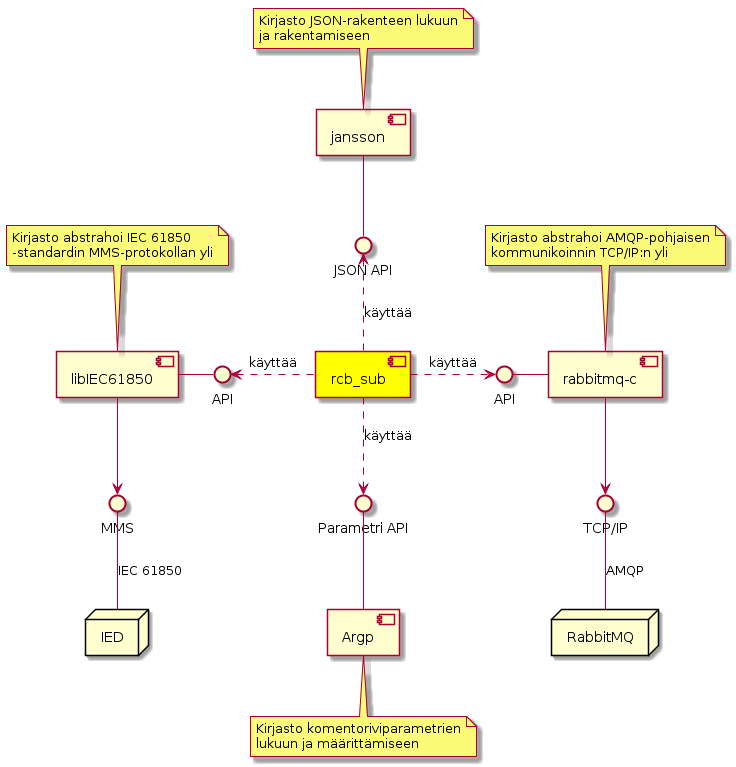
\includegraphics[width=1\textwidth]{pictures/rcb-sub-component-diagram.png}
	\caption{Toteutuksen komponenttikaavio sen osista ja relaatioista toisiinsa.}
	\label{fig:rcb-sub-komponenttikaavio}
\end{figure}

Toteutuksessa käytettiin seuraavia kirjastoja:
\begin{itemize}
	\item libiec61850,
	\item rabbitmq-c,
	\item jansson, ja
	\item Argp.
\end{itemize}
Kaikki käytetyt kirjastot on toteutettu C-kielellä, kuten rcb\_sub. Kirjastojen tarkoitus on abstrahoida jonkin asian käyttö ja tarjota käyttäjälle siitä helppokäyttöinen ja ymmärrettävä rajapinta. Rajapintaa käyttämällä kirjasto hoitaa matalan tason toiminnan ilman että kirjaston käyttäjän tarvitsee siitä välittää. Kirjasto libiec61850 abstrahoi IEC 61850 -standardin käyttöä ja hoitaa matalan tason MMS-protokollan kommunikoinnin \cite{libIEC61850-repo}. Samaa kirjastoa käytettiin ensimmäisessä demoversiossa (kappale \ref{ch:demoversio-ja-sen-toiminta}) ja kirjaston kerrosarkkitehtuuri oli esitetty kuvassa \ref{fig:libiec61850-layer-architecture}. Kuvassa \ref{fig:rcb-sub-komponenttikaavio} libiec61850 kommunikoi suoraan IED-laitteen kanssa MMS-protokollan yli. Kirjasto rabbitmq-c abstrahoi RabbitMQ-palvelimen käyttöä ja hoitaa matalan tason AMQP-pohjaisen kommunikoinnin \cite{rabbitmq-c-repo}. Toteutuksessa rabbitmq-c kommunikoi suoraan RabbitMQ-palvelimen kanssa. Kirjasto jansson abstrahoi JSON-rakenteiden lukua ja käsittelyä C-kielelle \cite{jansson-repo}. Kirjastoa käytettiin rakentamaan IED-laitteelta tulleesta viestistä JSON-muotoinen viesti. JSON-rakenne on nähtävissä liitteessä \ref{ch:report-json-format}. Kirjasto Argp auttaa ohjelman komentoriviparametrien määrittämisessä ja käsittelyssä \cite{argp-glibc-guide}. Kirjasto auttaa toteuttamaan ohjelmalle UNIX-tyyliset parametrit. Eli vaaditut parametrit ja vaihtoehtoiset lyhyet ja pitkä parametrit. Vaadituista parametreista esimerkiksi Linux:in komento \texttt{mv foo.txt bar.txt}, jossa foo.txt ja bar.txt ovat vaadittuja parametreja. Vaihtoehtoisista parametreista esimerkkinä pitkä muoto \texttt{-{}-bytes} ja lyhyt muoto \texttt{-b}. Lisäksi kirjasto lisää ohjelmaan automaattisesti Linux:ista käyttäjille tutut \texttt{-{}-help} ja \texttt{-{}-version} vaihtoehtoiset parametrit. Kommennolla \texttt{-{}-help} kirjasto tulostaa Linux:ilta tutun ohjelman aputeksin käyttäjälle, jossa on esitettu ohjelman kaikki parametrit ja niiden selitteet \cite{step-by-step-into-argp}.

\begin{it}
	Piirrä tähän sekvenssikaavio pääpiirteisestä toiminnasta ja käy se korkealla tasolla läpi. Tämän jälkeen tulevissa kappaleissa mennään tarkemmin toimintaa ohjelman ajojärjestuyksessä.
\end{it}


\section{Ohjelman toiminta}
\begin{it}
	Käsitele tässä alaotsikoilla järjestykessä kutakin kohtaa ohjelmasta tarkemmin kuinka se toimii. Käytä apuna UML-kaavioita ja koodiesimerkkejä toteutuksesta. Etene asiassa yleiskuvassa esitetyssä järjestykessä.
\end{it}


\subsection{Parametrisointi}


\subsection{IED:n attribuuttien määritysten luku}


\subsection{Viestien tilaus}


\subsection{JSON:nin muodostaminen}


\section{Jatkokehitys}
\begin{it}
	Kirjoita tähän ideoita mitä jää jatkokehitykseen ja mitä ohjelmistossa on puutteita tai mitä jäi tekemättä. Esim. testaus ja CMake lisääminen.
\end{it}